\documentclass{article}
\usepackage{amsmath}
\usepackage{graphicx}
\usepackage{float}
\usepackage{subcaption}
\usepackage{setspace}
\usepackage[backend=bibtex,style=verbose-trad2]{biblatex}
\usepackage{siunitx}
\usepackage{multirow}
\usepackage{booktabs}
\usepackage{tikz}
\usepackage{circuitikz}

\title{Test Document}
\author{Rayson Lim}
\date{27-12-2017}
\setcounter{tocdepth}{2}
\bibliography{My_Library}
\sisetup{
    round-mode = places,
    round-precision = 2
}
\usetikzlibrary{trees}

\begin{document}
    \pagenumbering{gobble}
    \maketitle
    \newpage
    \doublespacing
    \tableofcontents
    \singlespacing
    \newpage
    \pagenumbering{arabic}

    \section{Math Magic}

        \subsection{First Amazing Equation}
            \begin{equation}
            f(x) = x^2
            \end{equation}

        \subsection{Some Explaining To Do}
            Ever wondered why $f(x) = x^2$?\\
            Because
            \begin{align*}
            1 + 2 &= 3 \\
            1 &= 3 - 2 \\
            f(x) &= x^2 \\
            g(x) &= \frac{1}{x} \\
            F(x) &= \int^a_b \frac{1}{3}x^3
            \end{align*}

        \subsection{Playing With Matrice}
            $\begin{matrix}
            1 & 0 & 0 \\
            0 & 1 & 0 \\
            0 & 0 & 1
            \end{matrix}$

        \subsection{Random Einstein}
            \begin{figure}[H]
                \includegraphics[width=\linewidth]{Albert-Einstein.jpg}
                \caption{Best thinker of all time}
                \label{fig:einstein}
            \end{figure}

            Figure \ref{fig:einstein} shows my best friend (I wish). This is some example text \footnote{\label{myfootnote}I am the best}. Most random text to try and see if I can push the footnote label down. Over here, I am going to refer to \ref{myfootnote} again. 

            \subsubsection{Multiple Figures!}
                \begin{figure}[H]
                    \centering
                    \begin{subfigure}[b]{0.4\linewidth}
                        \includegraphics[width=\linewidth]{large_Space_Invader_Print_preview_featured.jpg}
                        \caption{Toilet Paper}
                    \end{subfigure}
                    \begin{subfigure}[b]{0.4\linewidth}
                        \includegraphics[width=\linewidth]{large_Space_Invader_Print_preview_featured.jpg}
                        \caption{More toilet paper}
                    \end{subfigure}

                    \begin{subfigure}[b]{0.7\linewidth}
                        \includegraphics[width=\linewidth]{large_Space_Invader_Print_preview_featured.jpg}
                        \caption{What is this?}
                    \end{subfigure}

                    \caption{So much toilet paper}
                    \label{fig:toilet_paper}
                \end{figure}
                This great example in figure \ref{fig:toilet_paper} shows how to make rows and columns. \autocite[1]{hunter_inside_2015}

    \section{More Features}
        \subsection{Table}
            \begin{table}[H]
                \begin{center}
                    \caption{Fake table}
                    \label{tab:table1}
                    \begin{tabular}{l|S|r}
                        \toprule
                        \textbf{Value 1} & \textbf{Value 2} & \textbf{Value 3}\\
                        $\alpha$ & $\beta$ & $\gamma$\\
                        \midrule
                        \multirow{2}{*}{1} & 1110.1 & a\\
                        & 10.1 & b\\
                        \midrule
                        3 & 23.113231 & c\\
                        4 & 33.11454 & d\\
                        \midrule
                        \multicolumn{2}{c|}{\multirow{2}{*}{5}} & e\\
                        \multicolumn{2}{c|}{} & f\\
                        \bottomrule
                    \end{tabular}
                \end{center}
            \end{table}

        \subsection{Drawing with Tikz}
            \begin{figure}[h!]
                \centering
                \begin{tikzpicture}
                    \draw [red,dashed] (-2.5,2.5) rectangle (-1.5,1.5) node [black,below] {Start};
                    \draw [thick] (-2,2)
                    to [out=10,in=180] (2,2)
                    to [out=0,in=90] (6,0)
                    to [out=-100,in=10](-2,-2);
                    \draw [black,fill] (5,0.1) rectangle (7,0) node [black,right] {Obstacle};
                    \draw [red,fill] (-2,-2) circle [radius=0.2] node [black,below=4] {Point of Interest};
                \end{tikzpicture}
                \caption{Nice path you got there!}
                \label{fig:path1}
            \end{figure}
            Lorem ipsum dolor sit amet, consectetur adipisicing elit, sed do eiusmod
            tempor incididunt ut labore et dolore magna aliqua. Ut enim ad minim veniam,
            quis nostrud exercitation ullamco laboris nisi ut aliquip ex ea commodo
            consequat. Duis aute irure dolor in reprehenderit in voluptate velit esse
            cillum dolore eu fugiat nulla pariatur. Excepteur sint occaecat cupidatat non
            proident, sunt in culpa qui officia deserunt mollit anim id est laborum.\\

        \subsection{Trees}
            \begin{figure}[H]
                \centering
                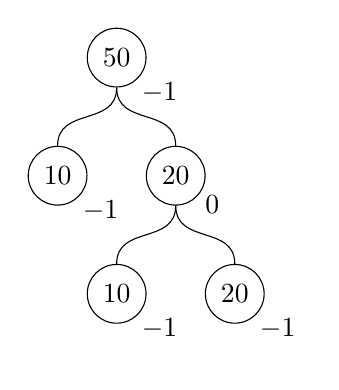
\begin{tikzpicture}[
                    edge from parent path={(\tikzparentnode.south)
                            .. controls +(0,-.5) and +(0,.5)
                            .. (\tikzchildnode.north)},
                    every node/.style={draw,circle},
                    label distance=-1mm]

                    \node [label=330:$-1$]{50}
                    child {node[label=330:$-1$] {10}}
                    child {node[label=330:$0$] {20}
                    child {node[label=330:$-1$] {10}}
                    child {node[label=330:$-1$] {20}}
                    };
                \end{tikzpicture}
                \caption{This syntax is so weird}
            \end{figure}
            Lorem ipsum dolor sit amet, consectetur adipisicing elit, sed do eiusmod
            tempor incididunt ut labore et dolore magna aliqua. Ut enim ad minim veniam,
            quis nostrud exercitation ullamco laboris nisi ut aliquip ex ea commodo
            consequat. Duis aute irure dolor in reprehenderit in voluptate velit esse
            cillum dolore eu fugiat nulla pariatur. Excepteur sint occaecat cupidatat non
            proident, sunt in culpa qui officia deserunt mollit anim id est laborum.\\

        \subsection{Probability Tree}
            \begin{figure}[H]
                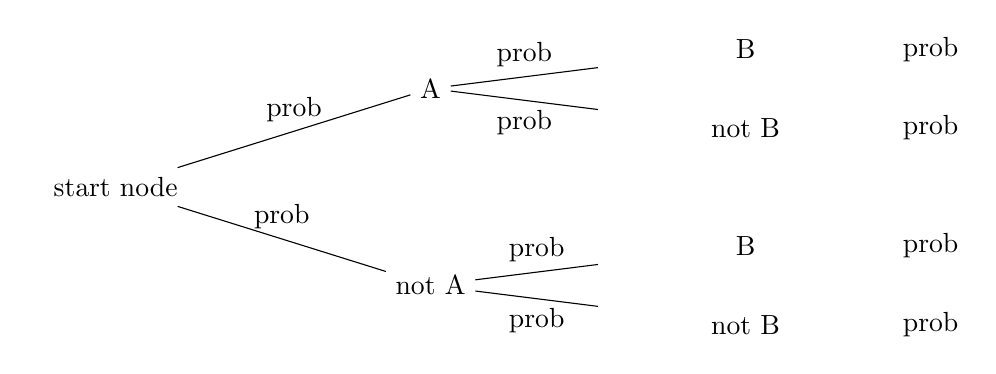
\begin{tikzpicture}[level distance = 4cm, grow=right]
                  \tikzstyle{level 1}=[sibling distance=2.5cm]
                  \tikzstyle{level 2}=[sibling distance=1cm]
                  \tikzstyle{en}=[text width=3.5cm, text centered]
                  \tikzstyle{start}=[text width=2cm, text centered]
                  
                  \node[start]{start node}
                    child{node{not A} 
                      child{node[en, label=right:prob]{not B}   edge from parent node[below]{prob}}
                      child{node[en, label=right:prob]{B}       edge from parent node[above]{prob}}
                      edge from parent node[above]{prob}
                    }
                    child{node{A} 
                      child{node[en, label=right:prob]{not B}   edge from parent node[below]{prob}}
                      child{node[en, label=right:prob]{B}       edge from parent node[above]{prob}}
                      edge from parent node[above]{prob}
                    }
                    ;
                \end{tikzpicture}
                \caption{Angie's pretty tree}
            \end{figure}
            Lorem ipsum dolor sit amet, consectetur adipisicing elit, sed do eiusmod
            tempor incididunt ut labore et dolore magna aliqua. Ut enim ad minim veniam,
            quis nostrud exercitation ullamco laboris nisi ut aliquip ex ea commodo
            consequat. Duis aute irure dolor in reprehenderit in voluptate velit esse
            cillum dolore eu fugiat nulla pariatur. Excepteur sint occaecat cupidatat non
            proident, sunt in culpa qui officia deserunt mollit anim id est laborum.\\

        \subsection{Circuits}
            \begin{figure}[H]
                \centering
                \begin{circuitikz}
                    \draw (0,0)
                    to[V,v=$U_q$] (0,2) % The voltage source
                    to[short] (2,2)
                    to[R=$R_1$] (2,0) % The resistor
                    to[short] (0,0);
                    \draw (2,2)
                    to[short] (4,2)
                    to[L=$L_1$] (4,0)
                    to[short] (2,0);
                    \draw (4,2)
                    to[short] (6,2)
                    to[C=$C_1$] (6,0)
                    to[short] (4,0);
                \end{circuitikz}
                \caption{First Circuit}
            \end{figure}

        \subsection{More Circuits!}
            \begin{figure}[H]
                \begin{circuitikz}
                    \draw (0,0)
                    to [short] node[ground]{GND} (0,-1);
                    \draw (0,0)
                    to [short] (8,0)
                    to [short] (8,2)
                    to [push button=Button A] (6,2)
                    to [short,-o] (6,2); 
                    \draw (8,2)
                    to [short] (8,4)
                    to [push button=Button B] (6,4)
                    to [short,-o] (6,4);

                    \draw (1,1) node[right=5]{From Mojo}
                    to [short,o-] (0,1)
                    to [leDo] (0,0);

                    \draw (1,3) node[right=5]{From Mojo}
                    to [short,o-] (0,3)
                    to [leDo] (0,2)
                    to [short] (-1,2)
                    to [short] (-1,0)
                    to [short] (0,0);
                \end{circuitikz}
            \end{figure}
    \newpage
    \section{Appendix}
    \begin{appendix}
        \listoffigures
        \listoftables
    \end{appendix}

    \newpage
    \section{Bibliography}
    \printbibliography

\end{document}